\documentclass[11pt,a4paper,spanish]{book}
\usepackage{estilo_unir-1}
\usepackage{tikz}
\usetikzlibrary{positioning, arrows.meta, decorations.pathmorphing, babel}
\usepackage{graphicx}



%---------------------------
%título del trabajo y autor
%---------------------------
\title{Oscilador armónico cuántico (OAC)}
\author{Nombre y Apellidos}
\date{diaXXX de mesXXX de 2023}
\profesor{Rodrigo Gil-Merino y Rubio}

%---------------------------
%marges
%---------------------------
%\usepackage[margin=1.9cm]{geometry}
%---------------------------
%---------------------------
%---------------------------
%---------------------------
\begin{document}
	\renewcommand{\listfigurename}{Índice de figuras}
	\renewcommand{\listtablename}{Índice de tablas}
	\renewcommand{\contentsname}{Índice de contenidos}
	\renewcommand{\figurename}{Figura}
	\renewcommand{\tablename}{Tabla} 
	
	\maketitle
	
	\frontmatter
	\tableofcontents
	\listoffigures %atención, quitar si no hay figuras!!!
	\listoftables %atención, quitar si no hay tablas!!!
	
	\chapter{Resumen}
	Aquí se introducirá un breve resumen en español del trabajo realizado (extensión máxima: 150 palabras). Este resumen debe incluir el objetivo o propósito de la investigación, la metodología, los resultados y las conclusiones (obviamente, todo muy resumido, pero así se sabe de un vistazo lo que se va uno a encontrar a continuación).\\
	
	
	{\bf Palabras clave:} se deben incluir de 3 a 5 palabras claves en español (pueden ser conceptos formados por más de una palabra)
	
	\chapter{Abstract}
	Aquí debe introducirse la versión en {\bf inglés} del Resumen anterior.\\
	
	
	{\bf Keywords:} se deben incluir de 3 a 5 palabras claves en inglés  (pueden ser conceptos formados por más de una palabra)
	
	
	
	
	\mainmatter
	
	
	
	\chapter{Desarrollo del Trabajo}
	
	\section{Solución del oscilador armónico cuántico}
	
	El oscilador armónico cuántico es uno de los pocos sistemas cuánticos con solución analítica exacta. En esta sección derivaremos tanto el espectro de energía como las autofunciones completas utilizando dos métodos complementarios: el método analítico de \cite{schrodinger1926b} (ecuación diferencial)  y el método algebraico de \cite{dirac1930} (operadores escalera). La equivalencia de ambos métodos valida la consistencia interna de la mecánica cuántica y demuestra que formalismos aparentemente diferentes describen la misma física subyacente.
	
	\subsection{Planteamiento del problema}
	
	Buscamos resolver la ecuación de Schrödinger independiente del tiempo \citep{schrodinger1926a}:
	
	\begin{equation}
		\hat{H}\psi(x) = E\psi(x)
	\end{equation}
	
	donde el hamiltoniano para una partícula de masa $m$ en un potencial armónico de frecuencia angular $\omega$ es:
	
	\begin{equation}
		\hat{H} = -\frac{\hbar^2}{2m}\frac{d^2}{dx^2} + \frac{1}{2}m\omega^2 x^2
	\end{equation}
	
	Esta forma del hamiltoniano combina el operador de energía cinética cuántico con el potencial clásico armónico $V(x) = \frac{1}{2}m\omega^2 x^2$ derivado de la ley de \cite{hooke1678}.
	
	Explícitamente, debemos resolver:
	
	\begin{equation}
		-\frac{\hbar^2}{2m}\frac{d^2\psi}{dx^2} + \frac{1}{2}m\omega^2 x^2 \psi(x) = E\psi(x)
		\label{eq:schrodinger_oac}
	\end{equation}
	
	\textbf{Condiciones de frontera:} Para que $\psi(x)$ sea normalizable y represente un estado físico, requerimos:
	
	\begin{equation}
		\lim_{x \to \pm\infty} \psi(x) = 0
	\end{equation}
	
	y
	
	\begin{equation}
		\int_{-\infty}^{\infty} |\psi(x)|^2 dx = 1
	\end{equation}
	
	\textbf{Objetivo:} Encontrar:
	\begin{enumerate}
		\item Los valores de energía $E_n$ permitidos (espectro)
		\item Las funciones de onda $\psi_n(x)$ correspondientes (autofunciones)
	\end{enumerate}
	
	Estos dos elementos constituyen la solución completa del problema cuántico.
	
	
\subsection{Solución algebraica mediante operadores}

El método algebraico, desarrollado por Dirac en "The Principles of Quantum Mechanics" (1930) \cite{dirac1930}, obtiene el espectro y estados del OAC sin resolver ecuaciones diferenciales, usando únicamente álgebra de operadores.

\subsubsection{Operadores de creación y aniquilación}

Definimos los operadores \cite{dirac1930}:

\begin{equation}
	\hat{a} = \sqrt{\frac{m\omega}{2\hbar}}\left(\hat{x} + \frac{i}{m\omega}\hat{p}\right)
\end{equation}

\begin{equation}
	\hat{a}^\dagger = \sqrt{\frac{m\omega}{2\hbar}}\left(\hat{x} - \frac{i}{m\omega}\hat{p}\right)
\end{equation}

Estos operadores no son hermitianos: $\hat{a}^\dagger \neq \hat{a}$.
De hecho, son adjuntos hermíticos entre sí: $(\hat{a})^\dagger = \hat{a}^\dagger$. Esto significa que \textbf{no representan observables físicos directamente}. Su utilidad es algebraica: actúan como operadores de ``escalera'' que permiten subir y bajar entre niveles de energía, sin ser ellos mismos cantidades medibles.

Sin embargo, combinaciones de $\hat{a}$ y $\hat{a}^\dagger$ pueden formar operadores hermitianos que sí son observables, como el operador número $\hat{N} = \hat{a}^\dagger\hat{a}$ o los operadores de posición y momento.\\

Podemos despejar estas relaciones para expresar $\hat{x}$ y $\hat{p}$ en términos de $\hat{a}$ y $\hat{a}^\dagger$:

\begin{align}
	\hat{x} &= \sqrt{\frac{\hbar}{2m\omega}}(\hat{a} + \hat{a}^\dagger) \\
	\hat{p} &= i\sqrt{\frac{m\omega\hbar}{2}}(\hat{a}^\dagger - \hat{a})
\end{align}

\subsubsection{Relación de conmutación fundamental}

De la relación de conmutación canónica de  \cite{born1925} $[\hat{x}, \hat{p}] = i\hbar$, derivamos (ver Apéndice~\ref{sec:born1925}):

\begin{equation}
	[\hat{a}, \hat{a}^\dagger] = 1
	\label{eq:conmutador}
\end{equation}

Esta es la relación fundamental que gobierna todo el sistema y es la base del álgebra bosónica desarrollada en el trabajo fundamental de Born, Heisenberg y Jordan \citep{bornheisenberg1926}.

\subsubsection{Factorización del hamiltoniano}

Sustituyendo las expresiones de $\hat{x}$ y $\hat{p}$ en el hamiltoniano:

\begin{align}
	\hat{H} &= \frac{\hat{p}^2}{2m} + \frac{1}{2}m\omega^2\hat{x}^2 \\
	&= \hbar\omega\left(\hat{a}^\dagger\hat{a} + \frac{1}{2}\right)
\end{align}

Definiendo el \textbf{operador número} \cite{dirac1930}:

\begin{equation}
	\hat{N} = \hat{a}^\dagger\hat{a}
\end{equation}

el hamiltoniano se escribe:

\begin{equation}
	\boxed{\hat{H} = \hbar\omega\left(\hat{N} + \frac{1}{2}\right)}
	\label{eq:hamiltoniano_factorizado}
\end{equation}

Esta factorización fue uno de los logros fundamentales del formalismo de \cite{dirac1930}.

\subsubsection{Derivación algebraica del espectro}
Buscamos estados con número definido de cuantos. Estos son \textbf{autoestados} del operador número $\hat{N}$: estados que permanecen iguales (salvo un factor numérico) cuando $\hat{N}$ actúa sobre ellos.

Supongamos que existe un autoestado $|n\rangle$ del operador número con autovalor $n$:

\begin{equation}
	\hat{N}|n\rangle = n|n\rangle
\end{equation}

Entonces, de la ecuación (\ref{eq:hamiltoniano_factorizado}):

\begin{equation}
	\hat{H}|n\rangle = \hbar\omega\left(n + \frac{1}{2}\right)|n\rangle
\end{equation}

Por lo tanto, el autovalor de energía es:

\begin{equation}
	E_n = \hbar\omega\left(n + \frac{1}{2}\right)
\end{equation}

Ahora debemos determinar qué valores puede tomar $n$.\\

\textbf{Propiedades de los operadores escalera:}

Usando la relación de conmutación (\ref{eq:conmutador}), se demuestra que (ver Apéndice~\ref{sec:normalizacion1}):

\begin{align}
	[\hat{N}, \hat{a}] &= -\hat{a} \\
	[\hat{N}, \hat{a}^\dagger] &= \hat{a}^\dagger
\end{align}

De estas relaciones se sigue que:

\begin{align}
	\hat{N}(\hat{a}|n\rangle) &= (n-1)(\hat{a}|n\rangle) \\
	\hat{N}(\hat{a}^\dagger|n\rangle) &= (n+1)(\hat{a}^\dagger|n\rangle)
\end{align}

\textbf{Interpretación:}
\begin{itemize}
	\item $\hat{a}^\dagger|n\rangle$ es autoestado de $\hat{N}$ con autovalor $n+1$ (operador de \emph{creación})
	\item $\hat{a}|n\rangle$ es autoestado de $\hat{N}$ con autovalor $n-1$ (operador de \emph{aniquilación})
\end{itemize}

Esta nomenclatura proviene de la interpretación de los operadores como creadores y destructores de cuantos de energía \citep{dirac1927}.\\

\textbf{Límite inferior:}

El autovalor de $\hat{N}$ satisface $\langle n|\hat{N}|n\rangle = \langle n|\hat{a}^\dagger\hat{a}|n\rangle = ||\hat{a}|n\rangle||^2 \geq 0$.

Por lo tanto, $n \geq 0$.

Debe existir un estado mínimo $|0\rangle$ tal que:

\begin{equation}
	\hat{a}|0\rangle = 0
\end{equation}

Este es el \textbf{estado vacío} o \textbf{estado fundamental} \citep{dirac1930}.

\textbf{Cuantización:} Aplicando sucesivamente $\hat{a}$ a cualquier estado, eventualmente llegamos al estado fundamental. Esto solo es posible si $n$ toma valores enteros:

\begin{equation}
	\boxed{n = 0, 1, 2, 3, \ldots}
\end{equation}


\subsubsection{Construcción de autoestados}

Todos los estados se construyen aplicando $\hat{a}^\dagger$ al vacío \citep{dirac1930}:

\begin{equation}
	|n\rangle = \frac{(\hat{a}^\dagger)^n}{\sqrt{n!}}|0\rangle
\end{equation}

La acción precisa de los operadores es (ver Apéndice~\ref{sec:normalizacion1}):

\begin{align}
	\hat{a}^\dagger|n\rangle &= \sqrt{n+1}|n+1\rangle \\
	\hat{a}|n\rangle &= \sqrt{n}|n-1\rangle
\end{align}

\begin{figure}[h]
	\centering
	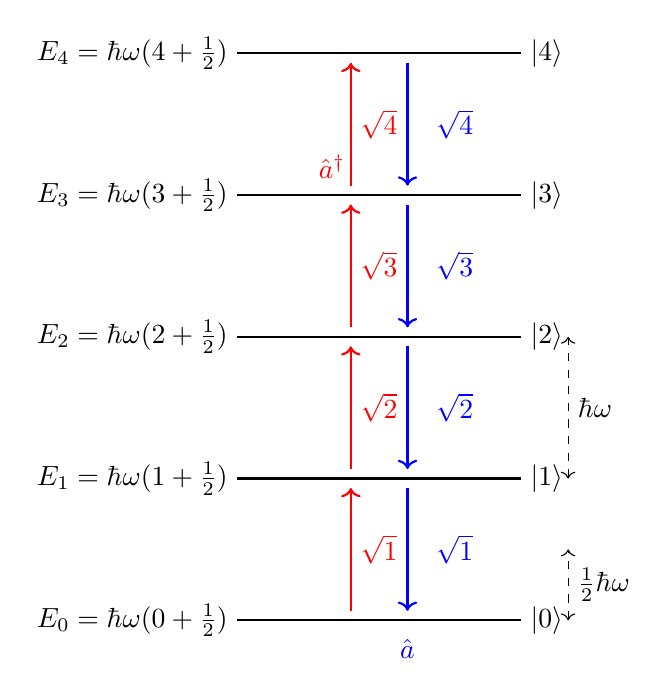
\begin{tikzpicture}[scale=1.2]
	% Niveles de energía
	\foreach \n in {0,1,2,3,4} {
		\draw[thick] (0,\n*1.5) -- (3,\n*1.5);
		\node[left] at (0,\n*1.5) {$E_{\n} = \hbar\omega(\n + \frac{1}{2})$};
		\node[right] at (3,\n*1.5) {$|{\n}\rangle$};
	}

	% Flechas de creación (rojas, hacia arriba)
\foreach \n in {0,1,2,3} {
	\pgfmathtruncatemacro{\m}{\n+1}
	\draw[->,red,thick] (1.2,\n*1.5+0.1) -- (1.2,\m*1.5-0.1);
	\node[red,right] at (1.2,\n*1.5+0.75) {$\sqrt{\m}$};
}
\node[red] at (1,4.8) {$\hat{a}^\dagger$};
		
		
		
		
		% Flechas de aniquilación (azules, hacia abajo)
	\foreach \n in {1,2,3,4} {
		\pgfmathtruncatemacro{\m}{\n-1}
		\draw[->,blue,thick] (1.8,\n*1.5-0.1) -- (1.8,\m*1.5+0.1);
		\node[blue,right] at (2,\n*1.5-0.75) {$\sqrt{\n}$};
	}
	\node[blue] at (1.8,-0.3) {$\hat{a}$};
	
	% Energía de punto cero
	\draw[<->,dashed] (3.5,0) -- (3.5,0.75);
	\node[right] at (3.5,0.375) {$\frac{1}{2}\hbar\omega$};
	\draw[<->,dashed] (3.5,1.5) -- (3.5,3);
	\node[right] at (3.5,2.25) {$\hbar\omega$};
	
\end{tikzpicture}

	\caption{Niveles de energía del oscilador armónico cuántico. Los operadores $\hat{a}^\dagger$ (rojo) y $\hat{a}$ (azul) actúan como escaleras, subiendo y bajando entre niveles con las constantes de normalización indicadas. El espaciado uniforme es $\hbar\omega$ y existe una energía de punto cero de $\frac{1}{2}\hbar\omega$. Fuente propia.}
	\label{fig:niveles}
\end{figure}



\subsection{Propiedades de las autofunciones}

\subsubsection{Autofunciones del oscilador armónico}

Los autoestados $|n\rangle$ obtenidos en la sección anterior son vectores abstractos en el espacio de Hilbert. Para calcular distribuciones de probabilidad y valores esperados de observables, necesitamos las \textbf{autofunciones} $\psi_n(x)$, que son las representaciones concretas de estos estados en el espacio de posición:

\begin{equation}
	\psi_n(x) = \langle x | n \rangle
\end{equation}

Las autofunciones son funciones de onda explícitas que podemos graficar y que satisfacen la ecuación de  \cite{schrodinger1926a} en forma de ecuación diferencial.

El resultado, derivado mediante el método analítico de \cite{schrodinger1926b} es:

\begin{equation}
	\psi_n(x) = \left(\frac{m\omega}{\pi\hbar}\right)^{1/4} \frac{1}{\sqrt{2^n n!}} H_n\left(\sqrt{\frac{m\omega}{\hbar}}x\right) \exp\left(-\frac{m\omega x^2}{2\hbar}\right)
	\label{eq:autofunciones}
\end{equation}

donde $H_n(\xi)$ son los polinomios de Hermite de orden $n$ (ver Apéndice~\ref{sec:hermite} para propiedades).


\subsubsection{Ortonormalidad}

Las autofunciones del oscilador armónico forman un conjunto \textbf{ortonormal}: son mutuamente ortogonales (perpendiculares en el sentido del producto interno) y cada una está normalizada (tiene norma unitaria). Matemáticamente:

\begin{equation}
	\int_{-\infty}^{\infty} \psi_n(x) \psi_m(x) dx = \delta_{nm}
\end{equation}

donde $\delta_{nm}$ es la delta de Kronecker:

\begin{equation}
	\delta_{nm} = \begin{cases} 
		1 & \text{si } n = m \\
		0 & \text{si } n \neq m
	\end{cases}
\end{equation}

\textbf{Ortogonalidad} ($n \neq m$): Funciones correspondientes a diferentes niveles de energía son mutuamente perpendiculares, reflejando que son estados físicamente distinguibles.

\textbf{Normalización} ($n = m$): Cada autofunción tiene probabilidad total igual a 1 de encontrar la partícula en algún lugar del espacio.


\subsubsection{Paridad}

Las funciones $\psi_n(x)$ tienen paridad bien definida:

\begin{equation}
	\psi_n(-x) = (-1)^n \psi_n(x)
\end{equation}

\textbf{Estados pares} ($n$ par): $\psi_n(-x) = +\psi_n(x)$ — función simétrica

\textbf{Estados impares} ($n$ impar): $\psi_n(-x) = -\psi_n(x)$ — función antisimétrica\\


\begin{figure}[h!]
	\centering
	
\includegraphics[width=1\linewidth]{paridad}
	\caption{Comparación paridad (estados pares vs impares). Fuente propia}
	\label{fig:paridad}
\end{figure}

\subsubsection{Número de nodos}

La función $\psi_n(x)$ tiene exactamente $n$ nodos (ceros):

\begin{itemize}
	\item $\psi_0(x)$: 0 nodos (gaussiana pura)
	\item $\psi_1(x)$: 1 nodo en $x = 0$
	\item $\psi_2(x)$: 2 nodos simétricos respecto al origen
	\item $\psi_n(x)$: $n$ nodos
\end{itemize}

Esta propiedad es general para problemas unidimensionales: el $n$-ésimo estado excitado tiene $n$ nodos.

\subsubsection{Funciones de onda de los primeros estados}

Usando la ecuación (\ref{eq:autofunciones}) y los primeros polinomios de Hermite (Apéndice ~\ref{sec:hermite}), obtenemos explícitamente:

\textbf{Estado fundamental ($n=0$):}
\begin{equation}
	\psi_0(x) = \left(\frac{m\omega}{\pi\hbar}\right)^{1/4} \exp\left(-\frac{m\omega x^2}{2\hbar}\right)
\end{equation}

Distribución gaussiana centrada en $x=0$ con ancho $\Delta x = \sqrt{\hbar/(2m\omega)}$.

\textbf{Primer estado excitado ($n=1$):}
\begin{equation}
	\psi_1(x) = \left(\frac{m\omega}{\pi\hbar}\right)^{1/4} \sqrt{\frac{2m\omega}{\hbar}} \, x \exp\left(-\frac{m\omega x^2}{2\hbar}\right)
\end{equation}

Función impar con un nodo en $x=0$.

\textbf{Segundo estado excitado ($n=2$):}
\begin{equation}
	\psi_2(x) = \left(\frac{m\omega}{\pi\hbar}\right)^{1/4} \frac{1}{\sqrt{2}}\left(\frac{2m\omega x^2}{\hbar} - 1\right) \exp\left(-\frac{m\omega x^2}{2\hbar}\right)
\end{equation}

Función par con dos nodos en $x = \pm\sqrt{\hbar/(2m\omega)}$.\\

\begin{table}[h]
	\centering
	\caption{Propiedades de los primeros estados del oscilador armónico cuántico}
	\label{tab:estados}
	\begin{tabular}{ccccl}
		\hline
		\textbf{Estado} & \textbf{Energía} & \textbf{Paridad} & \textbf{Nodos} & \textbf{Polinomio Hermite} \\
		$n$ & $E_n/(\hbar\omega)$ & Par/Impar & Cantidad & $H_n(\xi)$ \\
		\hline
		0 & 1/2 & Par & 0 & $1$ \\
		1 & 3/2 & Impar & 1 & $2\xi$ \\
		2 & 5/2 & Par & 2 & $4\xi^2 - 2$ \\
		3 & 7/2 & Impar & 3 & $8\xi^3 - 12\xi$ \\
		4 & 9/2 & Par & 4 & $16\xi^4 - 48\xi^2 + 12$ \\
		\hline
		\multicolumn{5}{l}{Patrón general: $E_n = \hbar\omega(n + \frac{1}{2})$, paridad = $(-1)^n$, nodos = $n$}
	\end{tabular}
\end{table}

	

\begin{figure}[h]
	\centering
	\includegraphics[width=0.8\linewidth]{"../ACTIVIDAD/Latex/funciones de onda"}
	\caption{Ejemplos de funciones de onda $\psi_0, \psi_1, \psi_2, \psi_3$. Fuente propia}
	\label{fig:funciones-de-onda}
\end{figure}



\begin{figure}[h!]
	\centering
	\includegraphics[width=0.8\linewidth]{"../ACTIVIDAD/Latex/densidad de onda"}
	\caption{Ejemplos de densidades de probaiblidad $|\Psi_n|$ }
	\label{fig:densidad-de-onda}
\end{figure}


\subsection{Equivalencia de ambos métodos}

Los métodos analítico y algebraico son completamente equivalentes, representando dos perspectivas complementarias del mismo sistema físico. La equivalencia fue demostrada explícitamente por \cite{schrodinger1926c} poco después de que \cite{dirac1925} introdujera el formalismo de operadores.

\subsubsection{Estado fundamental: comparación}

\textbf{Método analítico:} Para $n=0$, $H_0(\xi) = 1$, y la ecuación (\ref{eq:autofunciones}) da:

\begin{equation}
	\psi_0(x) = \left(\frac{m\omega}{\pi\hbar}\right)^{1/4} e^{-m\omega x^2/(2\hbar)}
\end{equation}

\textbf{Método algebraico:} La condición $\hat{a}|0\rangle = 0$ en representación de posición se traduce en:

\begin{equation}
	\sqrt{\frac{m\omega}{2\hbar}}\left(x + \frac{\hbar}{m\omega}\frac{d}{dx}\right)\psi_0(x) = 0
\end{equation}

Resolviendo esta ecuación diferencial ordinaria de primer orden:

\begin{equation}
	\frac{d\psi_0}{dx} = -\frac{m\omega}{\hbar} x \psi_0
\end{equation}

\begin{equation}
	\psi_0(x) = A e^{-m\omega x^2/(2\hbar)}
\end{equation}

Con normalización, $A = (m\omega/\pi\hbar)^{1/4}$.

\textbf{¡Ambos métodos dan la misma función!}

\subsubsection{Estados excitados: conexión}

En representación de posición, el operador $\hat{a}^\dagger$ actúa como \cite{dirac1930}:

\begin{equation}
	\hat{a}^\dagger \to \sqrt{\frac{m\omega}{2\hbar}}\left(x - \frac{\hbar}{m\omega}\frac{d}{dx}\right)
\end{equation}

Aplicando $(\hat{a}^\dagger)^n$ a $\psi_0(x)$ genera polinomios multiplicando la gaussiana, que son precisamente los polinomios de Hermite multiplicados por la constante apropiada \citep{sakurai2020}.

\subsubsection{Interpretación física}

\textbf{Método analítico \citep{schrodinger1926b}} :
\begin{itemize}
	\item Proporciona funciones de onda explícitas en representación de posición
	\item Visualización directa de densidades de probabilidad $|\psi_n(x)|^2$
	\item Útil para cálculos de valores esperados de observables
	\item Permite entender el comportamiento espacial de estados cuánticos
\end{itemize}

\textbf{Método algebraico \citep{dirac1930}} :
\begin{itemize}
	\item Más elegante y general
	\item No requiere resolver ecuaciones diferenciales
	\item Se generaliza fácilmente a otros sistemas
	\item Lenguaje natural para describir excitaciones (fonones, fotones) en sistemas de muchos cuerpos
	\item Fundamento de circuit QED y códigos bosónicos \citep{blais2021}
\end{itemize}

\begin{table}[h]
	\centering
	\caption{Comparación entre el método analítico (Schrödinger) y algebraico (Dirac)}
	\label{tab:comparacion_metodos}
	\begin{tabular}{p{4cm}p{5cm}p{5cm}}
		\hline
		\textbf{Aspecto} & \textbf{Método analítico} & \textbf{Método algebraico} \\
		\hline
		Formulación & Ecuación diferencial & Álgebra de operadores \\
		Herramienta principal & Polinomios de Hermite & Operadores escalera $\hat{a}$, $\hat{a}^\dagger$ \\
		Resultado directo & Autofunciones $\psi_n(x)$ & Espectro $E_n$ y autoestados $|n\rangle$ \\
		Complejidad matemática & Alta (EDOs, series) & Media (álgebra) \\
		Visualización & Directa ($|\psi_n(x)|^2$) & Requiere proyección \\
		Generalización & Específica al OAC & Se generaliza fácilmente \\
		\hline
	\end{tabular}
\end{table}


A lo largo de esta sección hemos derivado completamente el espectro de energía $E_n = \hbar\omega(n + \frac{1}{2})$ y las autofunciones $\psi_n(x)$ del oscilador armónico cuántico mediante el método desarrollado por \cite{dirac1930} y entendimos las equivalencias con el método desarrollado por \cite{schrodinger1926b}. La equivalencia matemática de ambos enfoques confirma la consistencia interna de la mecánica cuántica y demuestra que diferentes formalismos pueden describir el mismo sistema físico. Esta dualidad ha sido fundamental en el desarrollo de la física cuántica moderna, desde la teoría cuántica de campos hasta las aplicaciones contemporáneas en computación cuántica.
	
	
	\chapter{Conclusiones}
	
	Las Conclusiones es otra parte muy IMPORTANTE de la memoria. Deben ser muy clara. Si es posible se pueden itemizar o, mejor, poner un párrafo por idea con un pequeño título ilustrativo.
	
	\addcontentsline{toc}{chapter}{Bibliografía}
	\begin{thebibliography}{a}
		
		%% ORÍGENES CLÁSICOS Y PRE-CUÁNTICOS
		
		\bibitem[Hooke(1678)]{hooke1678} Hooke, R. (1678) \emph{Lectures de Potentia Restitutiva, or of Spring. Explaining the Power of Springing Bodies}. John Martyn, London.
		
		\bibitem[Lagrange(1788)]{lagrange1788} Lagrange, J.L. (1788) \emph{Mécanique analytique}. Desaint, Paris.
		
		\bibitem[Hamilton(1834)]{hamilton1834} Hamilton, W.R. (1834) On a General Method in Dynamics. \textit{Philosophical Transactions of the Royal Society}, Part I, 247--308.
		
		\bibitem[Hamilton(1835)]{hamilton1835} Hamilton, W.R. (1835) Second Essay on a General Method in Dynamics. \textit{Philosophical Transactions of the Royal Society}, Part I, 95--144.
		
		\bibitem[Wien(1896)]{wien1896} Wien, W. (1896) Über die Energievertheilung im Emissionsspectrum eines schwarzen Körpers. \textit{Annalen der Physik}, \textbf{294}(8), 662--669. DOI: 10.1002/andp.18962940803
		
		\bibitem[Rayleigh(1900)]{rayleigh1900} Rayleigh, J. W. S. (1900) Remarks upon the Law of Complete Radiation. \textit{Philosophical Magazine}, \textbf{49}, 539--540.
		
		\bibitem[Jeans(1905)]{jeans1905} Jeans, J.H. (1905) XI. On the Partition of Energy between Matter and Aether. \textit{The London, Edinburgh, and Dublin Philosophical Magazine and Journal of Science}, \textbf{10}, 91--98.
		
		\bibitem[Debye(1912)]{debye1912} Debye, P. (1912) Zur Theorie der spezifischen Wärmen. \textit{Annalen der Physik}, \textbf{39}(4), 789--839. DOI: 10.1002/andp.19123441404
		
		
		%% PAPERS SEMINALES HISTÓRICOS
		
		\bibitem[Planck(1901)]{planck1901} Planck, M. (1901) Über das Gesetz der Energieverteilung im Normalspektrum. \textit{Annalen der Physik}, \textbf{309}(3), 553--563. DOI: 10.1002/andp.19013090310
		
		\bibitem[Einstein(1907)]{einstein1907} Einstein, A. (1907) Die Plancksche Theorie der Strahlung und die Theorie der spezifischen Wärme. \textit{Annalen der Physik}, \textbf{22}, 180--190. DOI: 10.1002/andp.19063270110
		
		\bibitem[Heisenberg(1925)]{heisenberg1925} Heisenberg, W. (1925) Über quantentheoretische Umdeutung kinematischer und mechanischer Beziehungen. \textit{Zeitschrift für Physik}, \textbf{33}, 879--893. DOI: 10.1007/BF01328377
		
		\bibitem[Born \& Jordan(1925)]{born1925} Born, M. y Jordan, P. (1925) Zur Quantenmechanik. \textit{Zeitschrift für Physik}, \textbf{34}, 858--888.
		
		\bibitem[Born et al.(1926)]{bornheisenberg1926} Born, M., Heisenberg, W. y Jordan, P. (1926) Zur Quantenmechanik II. \textit{Zeitschrift für Physik}, \textbf{35}, 557--615.
		
		\bibitem[Schrödinger(1926a)]{schrodinger1926a} Schrödinger, E. (1926) Quantisierung als Eigenwertproblem (Erste Mitteilung). \textit{Annalen der Physik}, \textbf{384}(4), 361--376. DOI: 10.1002/andp.19263840404
		
		\bibitem[Schrödinger(1926b)]{schrodinger1926b} Schrödinger, E. (1926) Quantisierung als Eigenwertproblem (Zweite Mitteilung). \textit{Annalen der Physik}, \textbf{384}(6), 489--527. DOI: 10.1002/andp.19263840602
		
		\bibitem[Schrödinger(1926c)]{schrodinger1926c} Schrödinger, E. (1926) Der stetige Übergang von der Mikro- zur Makromechanik. \textit{Naturwissenschaften}, \textbf{14}, 664--666. DOI: 10.1007/BF01507634
		
		\bibitem[Dirac(1925)]{dirac1925} Dirac, P.A.M. (1925) The Fundamental Equations of Quantum Mechanics. \textit{Proceedings of the Royal Society of London A}, \textbf{109}, 642--653.
		
		\bibitem[Dirac(1927)]{dirac1927} Dirac, P.A.M. (1927) The Quantum Theory of the Emission and Absorption of Radiation. \textit{Proceedings of the Royal Society of London A}, \textbf{114}(767), 243--265.
		
		\bibitem[Dirac(1930)]{dirac1930} Dirac, P.A.M. (1930) \emph{The Principles of Quantum Mechanics}, 1st ed. Clarendon Press, Oxford.
		
		\bibitem[Glauber(1963a)]{glauber1963a} Glauber, R.J. (1963) The Quantum Theory of Optical Coherence. \textit{Physical Review}, \textbf{130}(6), 2529--2539. DOI: 10.1103/PhysRev.130.2529
		
		\bibitem[Glauber(1963b)]{glauber1963b} Glauber, R.J. (1963) Coherent and Incoherent States of the Radiation Field. \textit{Physical Review}, \textbf{131}(6), 2766--2788. DOI: 10.1103/PhysRev.131.2766
		
		\bibitem[Sudarshan(1963)]{sudarshan1963} Sudarshan, E.C.G. (1963) Equivalence of Semiclassical and Quantum Mechanical Descriptions of Statistical Light Beams. \textit{Physical Review Letters}, \textbf{10}(7), 277--279. DOI: 10.1103/PhysRevLett.10.277
		
		%% LIBROS DE TEXTO FUNDAMENTALES
		
		\bibitem[Griffiths \& Schroeter(2018)]{griffiths2018} Griffiths, D.J. y Schroeter, D.F. (2018) \emph{Introduction to Quantum Mechanics}, 3rd ed. Cambridge University Press, Cambridge.
		
		\bibitem[Sakurai \& Napolitano(2020)]{sakurai2020} Sakurai, J.J. y Napolitano, J. (2020) \emph{Modern Quantum Mechanics}, 3rd ed. Cambridge University Press, Cambridge.
		
		\bibitem[Cohen-Tannoudji et al.(2019)]{cohentannoudji2019} Cohen-Tannoudji, C., Diu, B. y Laloë, F. (2019--2020) \emph{Quantum Mechanics}, Vols. 1--3, 2nd ed. Wiley-VCH, Weinheim.
		
		\bibitem[Gerry \& Knight(2004)]{gerry2004} Gerry, C.C. y Knight, P.L. (2004) \emph{Introductory Quantum Optics}. Cambridge University Press, Cambridge.
		
		\bibitem[Nielsen \& Chuang(2010)]{nielsen2010} Nielsen, M.A. y Chuang, I.L. (2010) \emph{Quantum Computation and Quantum Information}, 10th Anniversary ed. Cambridge University Press, Cambridge.
		
		\bibitem[Schleich(2001)]{schleich2001} Schleich, W.P. (2001) \emph{Quantum Optics in Phase Space}. Wiley-VCH, Weinheim.
		
		\bibitem[Case(2008)]{case2008} Case, W.B. (2008) Wigner functions and Weyl transforms for pedestrians. \textit{American Journal of Physics}, \textbf{76}(10), 937--946.
		
		%% CIRCUIT QED Y QUBITS SUPERCONDUCTORES
		
		\bibitem[Koch et al.(2007)]{koch2007} Koch, J., Yu, T.M., Gambetta, J., Houck, A.A., Schuster, D.I., Majer, J., Blais, A., Devoret, M.H., Girvin, S.M. y Schoelkopf, R.J. (2007) Charge-insensitive qubit design derived from the Cooper pair box. \textit{Physical Review A}, \textbf{76}, 042319.
		
		\bibitem[Blais et al.(2004)]{blais2004} Blais, A., Huang, R.-S., Wallraff, A., Girvin, S.M. y Schoelkopf, R.J. (2004) Cavity quantum electrodynamics for superconducting electrical circuits: An architecture for quantum computation. \textit{Physical Review A}, \textbf{69}, 062320.
		
		\bibitem[Blais et al.(2021)]{blais2021} Blais, A., Grimsmo, A.L., Girvin, S.M. y Wallraff, A. (2021) Circuit quantum electrodynamics. \textit{Reviews of Modern Physics}, \textbf{93}, 025005.
		
		\bibitem[Wallraff et al.(2004)]{wallraff2004} Wallraff, A., Schuster, D.I., Blais, A., Frunzio, L., Huang, R.-S., Majer, J., Kumar, S., Girvin, S.M. y Schoelkopf, R.J. (2004) Circuit quantum electrodynamics: Coherent coupling of a single photon to a Cooper pair box. \textit{Nature}, \textbf{431}, 162--167.
		
		\bibitem[Krantz et al.(2019)]{krantz2019} Krantz, P., Kjaergaard, M., Yan, F., Orlando, T.P., Gustavsson, S. y Oliver, W.D. (2019) A quantum engineer's guide to superconducting qubits. \textit{Applied Physics Reviews}, \textbf{6}, 021318.
		
		%% IONES ATRAPADOS
		
		\bibitem[Cirac \& Zoller(1995)]{cirac1995} Cirac, J.I. y Zoller, P. (1995) Quantum computations with cold trapped ions. \textit{Physical Review Letters}, \textbf{74}, 4091--4094.
		
		\bibitem[Mølmer \& Sørensen(1999)]{molmer1999} Mølmer, K. y Sørensen, A. (1999) Multiparticle entanglement of hot trapped ions. \textit{Physical Review Letters}, \textbf{82}, 1835.
		
		\bibitem[Bruzewicz et al.(2019)]{bruzewicz2019} Bruzewicz, C.D., Chiaverini, J., McConnell, R. y Sage, J.M. (2019) Trapped-ion quantum computing: Progress and challenges. \textit{Applied Physics Reviews}, \textbf{6}, 021314.
		
		\bibitem[Leibfried et al.(2003)]{leibfried2003} Leibfried, D., Blatt, R., Monroe, C. y Wineland, D. (2003) Quantum dynamics of single trapped ions. \textit{Reviews of Modern Physics}, \textbf{75}, 281.
		
		%% CÓDIGOS BOSÓNICOS
		
		\bibitem[Gottesman et al.(2001)]{gkp2001} Gottesman, D., Kitaev, A. y Preskill, J. (2001) Encoding a qubit in an oscillator. \textit{Physical Review A}, \textbf{64}, 012310.
		
		\bibitem[Ofek et al.(2016)]{ofek2016} Ofek, N., Petrenko, A., Heeres, R., Reinhold, P., Leghtas, Z., Vlastakis, B., Liu, Y., Frunzio, L., Girvin, S.M., Jiang, L., Mirrahimi, M., Devoret, M.H. y Schoelkopf, R.J. (2016) Extending the lifetime of a quantum bit with error correction in superconducting circuits. \textit{Nature}, \textbf{536}, 441--445.
		
		\bibitem[Michael et al.(2016)]{michael2016} Michael, M.H., Silveri, M., Brierley, R.T., Albert, V.V., Salmilehto, J., Jiang, L. y Girvin, S.M. (2016) New class of quantum error-correcting codes for a bosonic mode. \textit{Physical Review X}, \textbf{6}, 031006.
		
		\bibitem[Campagne-Ibarcq et al.(2020)]{campagne2020} Campagne-Ibarcq, P., Eickbusch, A., Touzard, S., Zalys-Geller, E., Frattini, N.E., Sivak, V.V., Reinhold, P., Puri, S., Shankar, S., Schoelkopf, R.J., Frunzio, L., Mirrahimi, M. y Devoret, M.H. (2020) Quantum error correction of a qubit encoded in grid states of an oscillator. \textit{Nature}, \textbf{584}, 368--372.
		
		\bibitem[Sivak et al.(2023)]{sivak2023} Sivak, V.V., Eickbusch, A., Royer, B., Singh, S., Tsioutsios, I., Ganjam, S., Miano, A., Brock, B.L., Ding, A.Z., Frunzio, L., Girvin, S.M., Schoelkopf, R.J. y Devoret, M.H. (2023) Real-time quantum error correction beyond break-even. \textit{Nature}, \textbf{616}, 50--55. DOI: 10.1038/s41586-023-05782-6
		
		\bibitem[Ni et al.(2023)]{ni2023} Ni, Z., Li, S., Deng, X., Cai, Y., Zhang, L., Wang, W., Yang, Z.-B., Yu, H., Yan, F., Xu, S., Zhao, J.-S. y Zheng, D. (2023) Beating the break-even point with a discrete-variable-encoded logical qubit. \textit{Nature}, \textbf{616}, 56--60. DOI: 10.1038/s41586-023-05784-4
		
		\bibitem[Réglade et al.(2024)]{reglade2024} Réglade, U., Bocquet, A., Gautier, R., Cohen, J., Marquet, A., Albertinale, E., Pankratova, N., Hallén, M., Raskhodchikov, F., Jehl, L., Planat, L., Forment-Gillet, L., Esposito, M., Lescanne, R., Ficheux, Q., Mallet, F., Brune, M., Roch, N., Flurin, E., Huard, B., Leghtas, Z. y Devoret, M.H. (2024) Quantum control of a cat qubit with bit-flip times exceeding ten seconds. \textit{Nature}, \textbf{629}, 778--783. DOI: 10.1038/s41586-024-07294-3
		
		\bibitem[Putterman et al.(2025)]{putterman2025} Putterman, H., Noh, K., Xu, Q., Pereira, O., Ravi, G.S., Childs, J., Jiang, L., Albert, V.V. y Painter, O. (2025) Hardware-efficient quantum error correction using concatenated bosonic qubits. \textit{Nature}. DOI: 10.1038/s41586-025-08642-7
		
		\bibitem[Brady et al.(2024)]{brady2024} Brady, A.J., Kapourniotis, T. y Datta, A. (2024) Advances in Bosonic Quantum Error Correction with Gottesman-Kitaev-Preskill Codes. \textit{Progress in Quantum Electronics}, \textbf{93}, 100496.
		
		\bibitem[Terhal et al.(2020)]{terhal2020} Terhal, B.M., Conrad, J. y Vuillot, C. (2020) Towards scalable bosonic quantum error correction. \textit{Quantum Science and Technology}, \textbf{5}, 043001.
		
		%% TEORÍA CUÁNTICA DE CAMPOS
		
		\bibitem[Peskin \& Schroeder(1995)]{peskin1995} Peskin, M.E. y Schroeder, D.V. (1995) \emph{An Introduction to Quantum Field Theory}. Westview Press, Boulder.
		
			
		%% CVQC
		
		\bibitem[Braunstein \& van Loock(2005)]{braunstein2005} Braunstein, S.L. y van Loock, P. (2005) Quantum information with continuous variables. \textit{Reviews of Modern Physics}, \textbf{77}, 513--577.
		
		\bibitem[Weedbrook et al.(2012)]{weedbrook2012} Weedbrook, C., Pirandola, S., García-Patrón, R., Cerf, N.J., Ralph, T.C., Shapiro, J.H. y Lloyd, S. (2012) Gaussian quantum information. \textit{Reviews of Modern Physics}, \textbf{84}, 621.
		
		\bibitem[Madsen et al.(2022)]{madsen2022} Madsen, L.S., Laudenbach, F., Askarani, M.F., Rortais, F., Vincent, T., Bulmer, J.F.F., Miatto, F.M., Neuhaus, L., Helt, L.G., Collins, M.J., Lita, A.E., Gerrits, T., Nam, S.W., Vaidya, V.D., Menotti, M., Dhand, I., Vernon, Z., Quesada, N. y Lavoie, J. (2022) Quantum computational advantage with a programmable photonic processor. \textit{Nature}, \textbf{606}, 75--81.
		
		\bibitem[Bourassa et al.(2021)]{bourassa2021} Bourassa, J.E., Alexander, R.N., Vasmer, M., Patil, A., Tzitrin, I., Matsuura, T., Su, D., Baragiola, B.Q., Guha, S., Dauphinais, G., Sabapathy, K.K., Menicucci, N.C. y Dhand, I. (2021) Blueprint for a scalable photonic fault-tolerant quantum computer. \textit{Quantum}, \textbf{5}, 392.
		
		%% PAPERS EXPERIMENTALES RECIENTES
		
		\bibitem[Hou et al.(2024)]{hou2024} Hou, P.-Y., Nguyen, J.J., Kautz, L., Becker, B., Brocourt, L., Patel, R., Johansen, J., Sheremet, A. y Tan, T.R. (2024) Coherent coupling and non-destructive measurement of trapped-ion mechanical oscillators. \textit{Nature Physics}, \textbf{20}, 702--707. DOI: 10.1038/s41567-024-02599-6
		
		\bibitem[Hong et al.(1987)]{hong1987} Hong, C.K., Ou, Z.Y. y Mandel, L. (1987) Measurement of subpicosecond time intervals between two photons by interference. \textit{Physical Review Letters}, \textbf{59}(18), 2044--2046. DOI: 10.1103/PhysRevLett.59.2044
		
		\bibitem[Burd et al.(2024)]{burd2024} Burd, S.C., Srinivas, R., Knaack, H.M., Ge, W., Wilson, A.C., Wineland, D.J., Leibfried, D., Bollinger, J.J., Allcock, D.T.C. y Slichter, D.H. (2024) Squeezing-amplified interactions in quantum harmonic oscillators. \textit{PRX Quantum}, \textbf{5}, 020314. DOI: 10.1103/PRXQuantum.5.020314
		
		\bibitem[Park et al.(2024)]{park2024} Park, K., Kim, P. y Jeong, H. (2024) Experimental realization of entangled coherent states in two-dimensional harmonic oscillators of a trapped ion. \textit{Scientific Reports}, \textbf{14}, 7359. DOI: 10.1038/s41598-024-57391-6
		
		\bibitem[Dania et al.(2025)]{dania2025} Dania, L., Bykov, D.S., Conangla, G.P., Rieser, J., Quidant, R., Kiesel, N. y Novotny, L. (2025) High-purity quantum optomechanics at room temperature. \textit{Nature Physics}. DOI: 10.1038/s41567-025-02976-9
		
		\bibitem[Bild et al.(2023)]{bild2023} Bild, M., Fadel, M., Yang, Y., Schär, U., Chu, Y. y Yelin, S.F. (2023) Schrödinger cat states of a 16-microgram mechanical oscillator. \textit{Science}, \textbf{380}, 274--278. DOI: 10.1126/science.adf7553
		
		\bibitem[Piotrowski et al.(2023)]{piotrowski2023} Piotrowski, J., Windey, D., Vijayan, J., Gonzalez-Ballestero, C., de los Ríos Sommer, A., Meyer, N., Quidant, R., Romero-Isart, O., Reimann, R. y Novotny, L. (2023) Simultaneous ground-state cooling of two mechanical modes of a levitated nanoparticle. \textit{Nature Physics}, \textbf{19}, 1009--1013. DOI: 10.1038/s41567-023-01956-1
		
		\bibitem[Iyama et al.(2024)]{iyama2024} Iyama, D., Kamiya, T., Furusawa, S., Kanazawa, N., Kakuyanagi, K., Toida, H., Semba, K., Matsuzaki, Y., Munro, W.J. y Saito, S. (2024) Observation and manipulation of quantum interference in a superconducting Kerr parametric oscillator. \textit{Nature Communications}, \textbf{15}, 86. DOI: 10.1038/s41467-023-44496-1
		
		\bibitem[Wollack et al.(2022)]{wollack2022} Wollack, E.A., Cleland, A.Y., Gruenke, R.G., Wang, Z., Arrangoiz-Arriola, P. y Safavi-Naeini, A.H. (2022) Quantum state preparation and tomography of entangled mechanical resonators. \textit{Nature}, \textbf{604}, 463--467. DOI: 10.1038/s41586-022-04500-y
		
		\bibitem[Qiao et al.(2023)]{qiao2023} Qiao, H., Clerk, A.A. y Safavi-Naeini, A.H. (2023) Splitting phonons: building a platform for linear mechanical quantum computing. \textit{Science}, \textbf{380}, 1030--1033. DOI: 10.1126/science.adg8715
		
		\bibitem[Arrangoiz-Arriola et al.(2019)]{arrangoiz2019} Arrangoiz-Arriola, P., Wollack, E.A., Wang, Z., Pechal, M., Jiang, W., McKenna, T.P., Cleland, A.Y. y Safavi-Naeini, A.H. (2019) Resolving the energy levels of a nanomechanical oscillator. \textit{Nature}, \textbf{571}, 537--540. DOI: 10.1038/s41586-019-1386-x
		
		\bibitem[Grimm et al.(2020)]{grimm2020} Grimm, A., Frattini, N.E., Puri, S., Mundhada, S.O., Touzard, S., Mirrahimi, M., Girvin, S.M., Shankar, S. y Devoret, M.H. (2020) Stabilization and operation of a Kerr-cat qubit. \textit{Nature}, \textbf{584}, 205--209.
		
		\bibitem[Hajr et al.(2024)]{hajr2024} Hajr, A., Maiwöger, P., Renger, M., Albertinale, E., Banerjee, A., Reinhold, P., Leghtas, Z., Gross, R. y Fedorov, A. (2024) High-Coherence Kerr-Cat Qubit in 2D Architecture. \textit{Physical Review X}, \textbf{14}, 041049.
		
		\bibitem[Puri et al.(2019)]{puri2019} Puri, S., Boutin, S. y Blais, A. (2019) Stabilized cat in a driven nonlinear cavity: A fault-tolerant error syndrome detector. \textit{Physical Review X}, \textbf{9}, 041009.
		
		%% PERSPECTIVAS FUTURAS
		
		\bibitem[Liu et al.(2024)]{liu2024} Liu, Y., Griffin, P., Pittman, D., Smith, A., Chong, F.T., Martonosi, M. y Houck, A.A. (2024) Hybrid Oscillator-Qubit Quantum Processors: Instruction Set Architectures, Abstract Machine Models, and Applications. arXiv:2407.10381.
		
		\bibitem[Eickbusch et al.(2024)]{eickbusch2024} Eickbusch, A., Sivak, V., Ding, A.Z., Elder, S.S., Jha, S.R., Venkatraman, J., Royer, B., Girvin, S.M., Schoelkopf, R.J. y Devoret, M.H. (2024) Hardware-Efficient Fault Tolerant Quantum Computing with Bosonic Grid States in Superconducting Circuits. arXiv:2409.05813.
		
		\bibitem[Chamberland et al.(2022)]{chamberland2022} Chamberland, C., Noh, K., Arrangoiz-Arriola, P., Campbell, E.T., Hann, C.T., Iverson, J., Putterman, H., Bohdanowicz, T.C., Flammia, S.T., Keller, A., Refael, G., Preskill, J., Jiang, L., Safavi-Naeini, A.H., Painter, O. y Brandão, F.G.S.L. (2022) Building a fault-tolerant quantum computer using concatenated cat codes. \textit{PRX Quantum}, \textbf{3}, 010329.
		
		\bibitem[Alexander et al.(2025)]{alexander2025} Alexander, R.N., Yong, J.C., Bersin, E., Choi, H., Huber, J., Jaffe, M., Kaplan, A., Lauk, N., Ledford, J., Lo, A., Miller, S.A., Mondal, S., Phillips, M., Pooser, R., Spiropulu, M. y Verdon, G. (2025) Scaling and networking a modular photonic quantum computer. \textit{Nature}.
		
		%% BIBLIOGRAFÍA DEL APÉNDICE A
		
		\bibitem[Einstein(1907)]{einstein1907} Einstein, A. (1907) Die Plancksche Theorie der Strahlung und die Theorie der spezifischen Wärme. \textit{Annalen der Physik}, \textbf{22}, 180--190. DOI: 10.1002/andp.19063270110
		
		\bibitem[Debye(1912)]{debye1912} Debye, P. (1912) Zur Theorie der spezifischen Wärmen. \textit{Annalen der Physik}, \textbf{39}(4), 789--839. DOI: 10.1002/andp.19123441404
		
		\bibitem[Dulong \& Petit(1819)]{dulong1819} Dulong, P.L. y Petit, A.T. (1819) Recherches sur quelques points importans de la Théorie de la Chaleur. \textit{Annales de Chimie et de Physique}, \textbf{10}, 395--413.
		
	\end{thebibliography}
	%\bibliographystyle{plain} 
	%\bibliography{bibliografia}
	
	
	\appendix
	\chapter{Apéndices}

	
\section{Demostración de $[\hat{a}, \hat{a}^\dagger] = 1$} \label{sec:born1925}


Partimos de las definiciones:

\begin{align}
	\hat{a} &= \sqrt{\frac{m\omega}{2\hbar}}\left(\hat{x} + \frac{i}{m\omega}\hat{p}\right) \\
	\hat{a}^\dagger &= \sqrt{\frac{m\omega}{2\hbar}}\left(\hat{x} - \frac{i}{m\omega}\hat{p}\right)
\end{align}

Calculamos el conmutador $[\hat{a}, \hat{a}^\dagger] = \hat{a}\hat{a}^\dagger - \hat{a}^\dagger\hat{a}$:

\begin{align}
	\hat{a}\hat{a}^\dagger &= \frac{m\omega}{2\hbar}\left(\hat{x} + \frac{i}{m\omega}\hat{p}\right)\left(\hat{x} - \frac{i}{m\omega}\hat{p}\right) \\
	&= \frac{m\omega}{2\hbar}\left(\hat{x}^2 - \frac{i}{m\omega}\hat{x}\hat{p} + \frac{i}{m\omega}\hat{p}\hat{x} + \frac{1}{m^2\omega^2}\hat{p}^2\right) \\
	&= \frac{m\omega}{2\hbar}\hat{x}^2 + \frac{1}{2m\omega\hbar}\hat{p}^2 + \frac{i}{2\hbar}(\hat{p}\hat{x} - \hat{x}\hat{p})
\end{align}

El último término es $-\frac{i}{2\hbar}[\hat{x}, \hat{p}]$. Similarmente:

\begin{align}
	\hat{a}^\dagger\hat{a} &= \frac{m\omega}{2\hbar}\left(\hat{x} - \frac{i}{m\omega}\hat{p}\right)\left(\hat{x} + \frac{i}{m\omega}\hat{p}\right) \\
	&= \frac{m\omega}{2\hbar}\hat{x}^2 + \frac{1}{2m\omega\hbar}\hat{p}^2 + \frac{i}{2\hbar}[\hat{x}, \hat{p}]
\end{align}

Restando:

\begin{equation}
	[\hat{a}, \hat{a}^\dagger] = \hat{a}\hat{a}^\dagger - \hat{a}^\dagger\hat{a} = -\frac{i}{2\hbar}[\hat{x}, \hat{p}] - \frac{i}{2\hbar}[\hat{x}, \hat{p}] = -\frac{i}{\hbar}[\hat{x}, \hat{p}]
\end{equation}

Usando la relación de conmutación canónica de \cite{born1925}:

\begin{equation}
	[\hat{x}, \hat{p}] = i\hbar
\end{equation}

Obtenemos:

\begin{equation}
	[\hat{a}, \hat{a}^\dagger] = -\frac{i}{\hbar}(i\hbar) = -i^2 = 1
\end{equation}

\begin{equation}
	\boxed{[\hat{a}, \hat{a}^\dagger] = 1}
\end{equation}	
	
	


\section{Constantes de normalización: $\hat{a}^\dagger|n\rangle = \sqrt{n+1}|n+1\rangle$} \label{sec:normalizacion1}

Queremos determinar la constante de proporcionalidad cuando $\hat{a}^\dagger$ actúa sobre $|n\rangle$.

Sabemos que $\hat{a}^\dagger|n\rangle$ es proporcional a $|n+1\rangle$:

\begin{equation}
	\hat{a}^\dagger|n\rangle = c|n+1\rangle
\end{equation}

Para encontrar $c$, calculamos la norma al cuadrado:

\begin{equation}
	||\hat{a}^\dagger|n\rangle||^2 = \langle n|\hat{a}\hat{a}^\dagger|n\rangle
\end{equation}

Usando la relación de conmutación $\hat{a}\hat{a}^\dagger = \hat{a}^\dagger\hat{a} + 1$:

\begin{align}
	||\hat{a}^\dagger|n\rangle||^2 &= \langle n|(\hat{a}^\dagger\hat{a} + 1)|n\rangle \tag{A.14}\\
	&= \langle n|\hat{N}|n\rangle + \langle n|n\rangle \quad \text{(donde } \hat{N} = \hat{a}^\dagger\hat{a}\text{)} \tag{A.15}\\
	&= n + 1 \tag{A.16}
\end{align}

Por otro lado, si $\hat{a}^\dagger|n\rangle = c|n+1\rangle$:

\begin{equation}
	||\hat{a}^\dagger|n\rangle||^2 = |c|^2
\end{equation}

Igualando: $|c|^2 = n + 1$, entonces $c = \sqrt{n+1}$ (tomamos la raíz positiva por convención).

\textbf{Resultado:}

\begin{equation}
	\boxed{\hat{a}^\dagger|n\rangle = \sqrt{n+1}|n+1\rangle}
\end{equation}

	

\section{Constantes de normalización: $\hat{a}|n\rangle = \sqrt{n}|n-1\rangle$} \label{sec:normalizacion2}

De manera análoga, para $\hat{a}|n\rangle = d|n-1\rangle$:

\begin{align}
	||\hat{a}|n\rangle||^2 &= \langle n|\hat{a}^\dagger\hat{a}|n\rangle \\
	&= \langle n|\hat{N}|n\rangle \\
	&= n
\end{align}

Por lo tanto: $|d|^2 = n \implies d = \sqrt{n}$

\textbf{Resultado:}

\begin{equation}
	\boxed{\hat{a}|n\rangle = \sqrt{n}|n-1\rangle}
\end{equation}

\begin{table}[h]
	\centering
	\caption{Acción de los operadores escalera sobre autoestados}
	\label{tab:operadores_escalera}
	\begin{tabular}{ccc}
		\hline
		\textbf{Estado inicial} & \textbf{Operador creación} & \textbf{Operador aniquilación} \\
		& $\hat{a}^\dagger|n\rangle$ & $\hat{a}|n\rangle$ \\
		\hline
		$|0\rangle$ & $\sqrt{1}|1\rangle = |1\rangle$ & $0$ \\
		$|1\rangle$ & $\sqrt{2}|2\rangle$ & $\sqrt{1}|0\rangle = |0\rangle$ \\
		$|2\rangle$ & $\sqrt{3}|3\rangle$ & $\sqrt{2}|1\rangle$ \\
		$|3\rangle$ & $\sqrt{4}|4\rangle = 2|4\rangle$ & $\sqrt{3}|2\rangle$ \\
		$|n\rangle$ & $\sqrt{n+1}|n+1\rangle$ & $\sqrt{n}|n-1\rangle$ \\
		\hline
	\end{tabular}
\end{table}



\section{Polinomios de Hermite} \label{sec:hermite}

Los polinomios de Hermite $H_n(\xi)$ aparecen en las autofunciones del oscilador armónico cuántico. Este apéndice presenta sus propiedades esenciales.

\subsection{Definición}

Los polinomios de Hermite se definen mediante la fórmula de Rodrigues:

\begin{equation}
	H_n(\xi) = (-1)^n e^{\xi^2} \frac{d^n}{d\xi^n} e^{-\xi^2}
\end{equation}



\begin{figure}[h!]
	\centering
	
\includegraphics[width=0.9\linewidth]{../ACTIVIDAD/Latex/hermite}
	\caption{Ejemplos de Polinomios de Hermite $H_0, H_1, H_2, H_3$}
	\label{fig:hermite}
\end{figure}



\subsection{Primeros polinomios}

\begin{align}
	H_0(\xi) &= 1 \\
	H_1(\xi) &= 2\xi \\
	H_2(\xi) &= 4\xi^2 - 2 \\
	H_3(\xi) &= 8\xi^3 - 12\xi \\
	H_4(\xi) &= 16\xi^4 - 48\xi^2 + 12
\end{align}

\textbf{Propiedades generales:}
\begin{itemize}
	\item $H_n(\xi)$ es un polinomio de grado $n$
	\item El coeficiente del término de mayor grado es $2^n$
	\item Paridad: $H_n(-\xi) = (-1)^n H_n(\xi)$
\end{itemize}

\subsection{Relación de recurrencia}

Los polinomios se pueden generar mediante:

\begin{equation}
	H_{n+1}(\xi) = 2\xi H_n(\xi) - 2n H_{n-1}(\xi)
\end{equation}

Esta relación permite calcular $H_{n+1}$ conociendo $H_n$ y $H_{n-1}$.

\subsection{Ortogonalidad}

Los polinomios de Hermite son ortogonales con peso gaussiano:

\begin{equation}
	\int_{-\infty}^{\infty} H_n(\xi) H_m(\xi) e^{-\xi^2} d\xi = \begin{cases}
		0 & \text{si } n \neq m \\
		\sqrt{\pi} \, 2^n n! & \text{si } n = m
	\end{cases}
\end{equation}

Esta propiedad garantiza la ortonormalidad de las autofunciones del OAC cuando se incluye la constante de normalización apropiada:

\begin{equation}
	A_n = \left(\frac{m\omega}{\pi\hbar}\right)^{1/4} \frac{1}{\sqrt{2^n n!}}
\end{equation}

\subsection{Consecuencias para las autofunciones}

\textbf{Paridad:} Como $H_n(-\xi) = (-1)^n H_n(\xi)$, las autofunciones tienen paridad bien definida:
\begin{equation}
	\psi_n(-x) = (-1)^n \psi_n(x)
\end{equation}

Estados pares ($n$ par): funciones simétricas

Estados impares ($n$ impar): funciones antisimétricas

\textbf{Número de nodos:} El polinomio $H_n(\xi)$ tiene exactamente $n$ ceros reales. Por lo tanto, $\psi_n(x)$ tiene exactamente $n$ nodos.



	
\end{document}